\documentclass{article}
\usepackage{arxiv}

\usepackage[utf8]{inputenc}
\usepackage[english]{babel}
\usepackage[T1]{fontenc}
\usepackage{url}
\usepackage{booktabs}
\usepackage{amsfonts}
\usepackage{nicefrac}
\usepackage{microtype}
\usepackage{lipsum}
\usepackage{graphicx}
%\usepackage{natbib}
\usepackage{doi}
\usepackage{svg}

\usepackage{amsmath}
\DeclareMathOperator*{\argmax}{arg\,max}
\DeclareMathOperator*{\argmin}{arg\,min}



\title{Image Style Transfer for Distillation of Diffusion Knowledge into a Transformer}

\author{ Egor Y.~Silvestrov \\
	Faculty of Computational Mathematics and Cybernetics \\
	Lomonosov Moscow State University \\
	Moscow, Russia \\
	\texttt{s02210546@gse.cs.msu.ru} \\
	%% examples of more authors
	\And
        Victor V.~Kitov \\
	Faculty of Computational Mathematics and Cybernetics \\
	Lomonosov Moscow State University \\
	Moscow, Russia \\
	\texttt{v.v.kitov@yandex.ru} \\
	%% \AND
	%% Coauthor \\
	%% Affiliation \\
	%% Address \\
	%% \texttt{email} \\
	%% \And
	%% Coauthor \\
	%% Affiliation \\
	%% Address \\
	%% \texttt{email} \\
	%% \And
	%% Coauthor \\
	%% Affiliation \\
	%% Address \\
	%% \texttt{email} \\
}
\date{}

\renewcommand{\shorttitle}{Image Style Transfer for Distillation of Diffusion Knowledge into a Transformer}

%%% Add PDF metadata to help others organize their library
%%% Once the PDF is generated, you can check the metadata with
%%% $ pdfinfo template.pdf
\hypersetup{
pdftitle={A template for the arxiv style},
pdfsubject={q-bio.NC, q-bio.QM},
pdfauthor={Egor Y.~Silvestrov, Victor V.~Kitov},
pdfkeywords={},
}

\begin{document}
\maketitle

\begin{abstract}
	Modern methods of style transfer for weak models often face problems with the quality of style transfer, especially in conditions of limited computing resources and untagged data (unsupervised learning). Distilling knowledge through diffusion models is a promising approach to improve the quality of weak models by transferring key elements of knowledge from more powerful models by creating a marked-up dataset and turning an unsupervised task into a supervised task with a teacher. In this paper, we investigate the method of distilling knowledge for a diffusion model, which allows us to adapt the styling and transmission of content for a more lightweight model (based on the transformer architecture) without the need for significant computational costs. As a result, an optimal balance is achieved between maintaining high-quality visual characteristics and cost-effectiveness, which opens up new opportunities for developing effective stylization models in real time.
\end{abstract}


\keywords{Image Style Transfer \and Diffusion Model \and Knowledge Distillation \and Transformer}

\section{Introduction}
    Image style transfer has gained significant attention in the creation of artistic visuals. The task involves taking a content image and a style reference image to produce an output that retains core content elements while adopting the visual style of the reference. This technique has applications across various domains, such as clothing design \cite{method 6}, photo and video editing \cite{method 7, method 8}, virtual reality \cite{method 9}, and more. Recently, deep neural networks have been widely used for style transfer, which can be grouped into three main approaches: 1) optimization-based methods, 2) feedforward approximation, and 3) zero-shot style transfer. Gates et al. \cite{method 10} proposed optimizing pixel values in a content image by minimizing both feature reconstruction and style losses, producing impressive results but requiring multiple iterations for each content-style pair, making it computationally expensive. In response, feedforward networks \cite{method 11, method 12, method 13} were developed to directly learn mappings from photographs to stylized images in specific painting styles, although retraining is required for new styles. Zero-shot style transfer is more versatile, as it can handle diverse styles, even previously unseen ones. Huang et al. \cite{method 14} introduced an arbitrary style transfer approach using adaptive instance normalization (AdaIN), which normalizes content image features and adjusts them based on style parameters. Recent work replaces AdaIN with whitening and coloring transformations \cite{method 15}, while several studies further refine this approach \cite{method 16, method 17}.
    
    However, a common limitation of these methods is that merely adjusting feature statistics makes it difficult to synthesize complex style patterns rich in detail and local structures, often resulting in distorted and less recognizable images. For instance, methods by Gatys et al. \cite{method 10}, AdaIN \cite{method 14}, and WCT \cite{method 15} frequently introduce style distortions that blur original content details. To address this, Deng et al. developed StyTr2 \cite{method 18}, which uses attention to capture semantic correlations between content and style features, yielding visually appealing results. Nevertheless, StyTr2 also suffers from structure distortion due to its shallow feature extractor, which lacks pre-trained weights, limiting its ability to differentiate between foreground and background objects. Thus, achieving a representation that can maintain content structure while accurately capturing fine-grained style patterns remains a challenging problem.
    
    Diffusion models \cite{method 1, method 2, method 3, method 4} have also achieved remarkable success in style transfer, excelling at generating visually coherent and detailed stylizations. In this paper, we propose using STTR \cite{method 5}, a Transformer-based model, as a student model to distill knowledge from a larger diffusion model \cite{method 4}. This diffusion model was taken based on good experimental results and the existence of an implementation. In this setup, the diffusion model \cite{method 4} performs style transfer on images, and STTR \cite{method 5} is trained to replicate these stylized outputs, effectively reframing style transfer as a supervised learning task. Transformer-based architectures, popularized by advancements in natural language processing \cite{method 19}, have demonstrated effectiveness in vision tasks by modeling long-range dependencies. The STTR \cite{method 5} approach uses to decompose content and style images into visual tokens, enabling learning of the global context between them. As similar content tokens align with the corresponding style tokens, this approach achieves detailed style transformation with structural consistency between content and style.

    We believe that training a small, relatively diffusive transformer model will allow us to achieve the quality of large diffusive models while using much fewer resources, which allows us to run this model on various low-power devices.

\section{Problem Statement}
\label{sec:ps}
Transferring the image style in a more general setting requires using the input image of the content $X_{c}$ and the input image of the style $X_{s}$ to obtain a stylized image of the content with this style $\hat{X_{t}}$.
This task can be described as follows:
$$ f_{\theta}(X_{c},X_{s}) = \hat{X_{t}}, $$ where $f_{\theta}(\cdot, \cdot)$ is the model and $\theta$ is its parameters.
Neural networks are used as models. This task is usually an unsupervised task and is solved with the help of specially selected loss functions. Completely different architectures are used, which are trained using iterative optimization methods (SGD for example).

Recently, diffusion models do a good job with this task, but they are very heavy and expensive to calculate, so in the current article this task becomes a supervised task, since the knowledge of the diffusion model is distilled into a smaller model (transformer) optimizing the loss function:
$$ \underset{X_{t} \sim P(X_{t})}{\mathrm{argmin}}\mathbb{E}L(\hat{X_{t}}, X_{t}),$$
where $X_{t}$ is the result of the diffusion model, $\hat{X_{t}}$ is the result of the student (transformer) model and $P(X_{t})$ is distribution of diffusion model results $X_{t}$. Loss functions are related to the sum of squared errors, and specific types of loss functions described in the section \ref{sec:experimetns}.

It is necessary to find such a model so that it is as simple as possible (since there is a need to run it on various devices) and of the highest quality in terms of the loss function, since there is no objective criterion for evaluating the results of stylization in this area.

Diffusion models require pre-trained Stable Diffusion weights, so they weigh at least 4GB already, but they also require computing power, which users usually do not have, and since the process in the diffusion model is iterative, it also takes time. Our goal is to offer a lighter transformer, which may be able to be run locally by most users, but which was able to get the quality attached to the diffusion model.

\section{Method}
\label{sec:methods}
\subsection{Overview}
Based on the experiments of choosing a diffusion model (in section \ref{sec:experimetns_choosing_diff}), the model from \cite{method 4} was taken as a teacher model. Since the result of the diffusion model is quite specific, in order to capture complex patterns, it is proposed to use complex models too, but smaller in size - transformers. Model \cite{method 5} was taken as a student model, it was chosen based on the benchmarks in the articles and the ease of code implementation.

\subsection{Architecture}
\paragraph{Student's Architecture} This model for fine-grained image style transfer using visual transformers. The architecture utilizes a combination of transformer-based encoders to extract semantic content and stylistic features separately. A specialized module aligns these features to synthesize the stylized image, preserving fine-grained details while maintaining semantic consistency. It integrates adaptive attention mechanisms for better content-style fusion, ensuring high-quality outputs. For more detailed specifics on layers and implementation, you can consult the original paper here \cite{method 5}.

\paragraph{Teacher's Architecture} The model described in the paper uses a "style injection" mechanism for adapting large-scale diffusion models to style transfer tasks. This approach is training-free and involves modifying intermediate layers of pre-trained diffusion models to encode style-specific features. By adjusting the feature maps during the reverse diffusion process, the model achieves style transfer while maintaining the original image content. The architecture leverages attention mechanisms and pre-trained weights from existing diffusion models, ensuring high-quality results without additional fine-tuning. You can explore more details in the full paper \cite{method 4}.


\subsection{Objective Function}
The VGG19 model \cite{method 20} was used to calculate some loss functions. In the experiments section \ref{sec:experimetns_choosing}, 3 objective functions were tried and as a result, the MSE function gave the best results:
$$ L(\hat{X_{t}}, X_{t}) = ||\hat{X_{t}} - X_{t} ||^2_{l_2}.$$


\subsection{Dataset Creating}
For training, images of content from the \texttt{COCO 2014 Dataset (for YOLOv3)} were used, so that the model immediately learns to correctly style faces (as the diffusion model does), the \texttt{Human Faces} dataset was used, and the \texttt{WikiArt} dataset was used for style. Depending on the experiment, the data were different, but the general rule was followed: two images with random faces were added to 10 images of random content and 8 random styles were selected; all images were scaled to a size of $512\times512$ and if the image is not square, then the edges were cut off, run through a diffusion model and a total of $(10 + 2) \cdot 8 = 96$ target $512\times512$ images for each combination of 10-2-8 were obtained.

For visual testing of the operation of various pipelines, a golden set of 7 content images and 6 style cutouts was selected, on which no pipeline was trained or validated. All the pictures with the result of the work were taken from a gold set.


\section{Experiments}
\begin{figure}[h]
    \centering
    \includegraphics[width=0.7\textwidth]{compare_diffs_1.png}
    \caption{The result of comparing two diffusion models:Inversion-based Style Transfer with Diffusion Models and Style Injection in Diffusion.}\label{fig:compare_diffs_models}
\end{figure}
\label{sec:experimetns}
\subsection{Choosing a Teacher Model}
Of the popular image style transfer diffusion models \cite{method 1,method 2, method 4}, only \cite{method 2, method 4} have been tested, since they have an implementation code in the public domain. The problem with model \cite{method 2} was that it generated images with style elements that were not in the style picture, that is, the model generated new content based on its knowledge. This effect is bad in the case of distilling knowledge into a transformer, since it has much fewer weights and it will not be able to remember the elements of various styles inside them. Method \cite{method 4} works more like all classical approaches of transferring the image style, trying only to extract dependencies for content from the current style image and it is better suited for distillation, therefore it is used as a teacher model. 

For example, if we look at Figure \ref{fig:compare_diffs_models}, we can see that the face on the left has acquired new features that are not in the style picture, but these features are in the same spirit and information about stylization is taken from the scales of the diffusion model, in the right picture the result of stylization without new elements.

\label{sec:experimetns_choosing_diff}
\subsection{Choosing Objective Function}
\label{sec:experimetns_choosing}
\begin{figure}[h]
    \centering
    \includegraphics[width=0.7\textwidth]{compares_2.png}
    \caption{Comparison of 3 objective functions on a golden dataset. SIID is Style Transfer with Diffusion Models from \cite{method 4} and STTR is STyle TRansformer from \cite{method 5}.}\label{fig:compare_diffs_models_2}
\end{figure}

Several different types of loss functions were tried for experiments, but only the selected three gave significantly different results:
\begin{equation}\label{eq:l1} L_{1}(\hat{X_{t}}, X_{t}) = ||\hat{X_{t}} - X_{t} ||^2_{l_2}, \end{equation}


\begin{equation}\label{eq:l2} L_{2}(\hat{X_{t}}, X_{t}) = 0.5 \cdot||\hat{X_{t}} - X_{t} ||^2_{l_2} + 0.5 \cdot \Sigma_{i=1}^{4}||\Phi(F_{i}(\hat{X_{t}})) - \Phi(F_{i}(X_{t}))||^2_{l_2}, \end{equation}

\begin{equation}\label{eq:l3} L_{3}(\hat{X_{t}}, X_{t}) = 0.7 \cdot||\hat{X_{t}} - X_{t} ||^2_{l_2} + 0.3 \cdot \Sigma_{i=1}^{4}||\Phi(F_{i}(\hat{X_{t}})) - \Phi(F_{i}(X_{t}))||^2_{l_2}, \end{equation}

where $F_{1}(X)$ is the activation slice from the 1st to the 2nd layer of VGG19, $F_{2}(X)$ is the activation slice from the 3rd to the 7th layer of VGG19, $F_{3}(X)$ is the activation slice from the 8th to the 12th layer of VGG19, $F_{4}(X)$ is the activation slice from the 13th to the 21st layer of VGG19, $\Phi(X)$ calculates the gram matrix for the input $X$. 

A total of \textbf{8,700} examples were generated, of which \textbf{7800}, \textbf{900} examples went to the training set for validation for the training step. The training for each loss was carried out under the same conditions, all the seeds were fixed. In model \cite{method 5}, everything was trained except the layer with VGG19, which was used for the loss function. The motivation behind Formula \ref{eq:l1} is to offer to try one of the easiest ways to learn for a supervised task. The motivation of formula \ref{eq:l2} follows from the author of \cite{method 5}, who solved the unsupervised task using a similar loss function. Formula \ref{eq:l3} is a modification of formula \ref{eq:l2}, with a large weight of simple repetition, since we noticed that a defect appeared with the loss function \ref{eq:l2} and focused on simply repeating the teacher's picture through MSE loss. The training started with pre-trained weights of the model \cite{method 5}. For all loss functions, training stopped after reducing the step did not help to reduce the loss further during 3-4 validation epochs.

\subsection{Summary}
Some of the results of the work on the gold set can be seen in Figure \ref{fig:compare_diffs_models_2}. The general properties for the learning result are that the model has lost the defects of the picture and the colours of the image began to adjust to the result of the teacher's work. The content tends to be preserved, and the style is applied mainly in colour. Loss $L_{2}$ has a problem, since its result is less saturated with the colour of the style, and also has more defects than loss $L_1$ and $L_3$. $L_1$ and $L_3$ are mostly different in brightness and $L_1$ is brighter, so this option is the best among the others.
\subsection{Discussions}
Within the framework of this study, the task was set to distil the knowledge of the diffusion model into the transformer architecture for the task of transferring style using images as a source of style.

The proposed approach demonstrates a tendency to transfer the colour characteristics of the style, which meets the expectations for stylization tasks, an analogue of repainting objects using segmentation. Nevertheless, the structure of the original image is preserved much more strongly (this is the weak side of the proposed approach) than in the original (non-distilled) diffusion model. This may be due to the fact that the transformer, due to simplified representation and training on preprocessed data, captures textural or spatial features of the style less successfully.

\section{Conclusion}
\label{sec:conclusion}
When distilling model \cite{method 4} into model \cite{method 5}, defects disappear from model \cite{method 4} and it transmits colours more correctly, however, the disadvantage is that it practically does not change the content for the style structure, but we got a model that weighs 10 times less and can run on a much larger number of video cards. in further studies, we want to try other architectures for the student's prayer and various variants of the object function.

% \section{Examples of citations, figures, tables, references}
% \label{sec:others}

% \subsection{Citations}
% Citations use \verb+natbib+. The documentation may be found at
% \begin{center}
% 	\url{http://mirrors.ctan.org/macros/latex/contrib/natbib/natnotes.pdf}
% \end{center}

% Here is an example usage of the two main commands (\verb+citet+ and \verb+citep+): Some people thought a thing \citep{kour2014real, hadash2018estimate} but other people thought something else \citep{kour2014fast}. Many people have speculated that if we knew exactly why \citet{kour2014fast} thought this\dots

% \subsection{Figures}
% \lipsum[10]
% See Figure \ref{fig:fig1}. Here is how you add footnotes. \footnote{Sample of the first footnote.}
% \lipsum[11]

% \begin{figure}
% 	\centering
% 	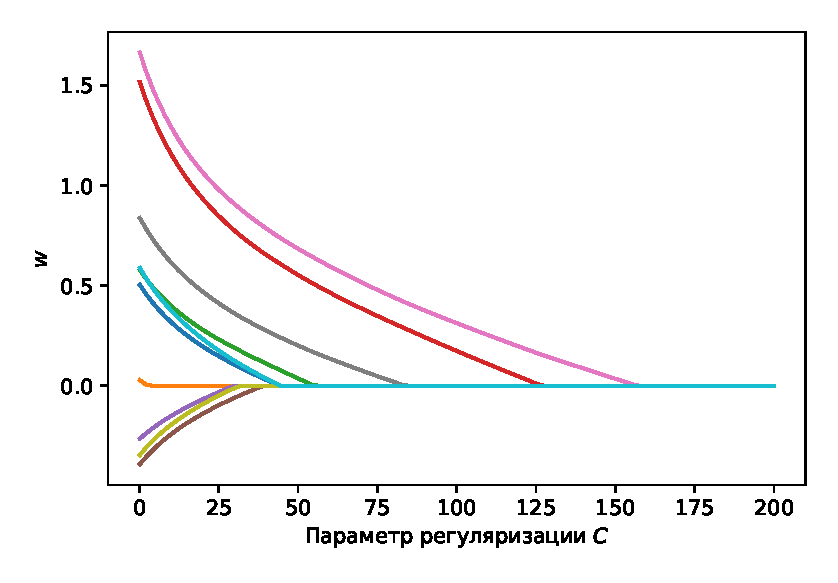
\includegraphics[width=0.5\textwidth]{../figures/log_reg_cs_exp.eps}
% 	\caption{Sample figure caption.}
% 	\label{fig:fig1}
% \end{figure}

% \subsection{Tables}
% See awesome Table~\ref{tab:table}.

% The documentation for \verb+booktabs+ (`Publication quality tables in LaTeX') is available from:
% \begin{center}
% 	\url{https://www.ctan.org/pkg/booktabs}
% \end{center}


% \begin{table}
% 	\caption{Comparison of models by memory.}
% 	\centering
% 	\begin{tabular}{lll}
% 		\toprule
% 		\multicolumn{2}{c}{Part}                   \\
% 		\cmidrule(r){1-2}
% 		Name     & Description     & Size ($\mu$m) \\
% 		\midrule
% 		STTR & Input terminal  & 519 Mb     \\
% 		Inversion-based Style Transfer with Diffusion Models     & Output terminal &      \\
% 		Soma     & Cell body       & up to $10^6$  \\
% 		\bottomrule
% 	\end{tabular}
% 	\label{tab:table}
% \end{table}

% \subsection{Lists}
% \begin{itemize}
% 	\item Lorem ipsum dolor sit amet
% 	\item consectetur adipiscing elit.
% 	\item Aliquam dignissim blandit est, in dictum tortor gravida eget. In ac rutrum magna.
% \end{itemize}


% \bibliographystyle{unsrtnat}
% \bibliography{references.bib}


\renewcommand{\bibname}{References}
\addcontentsline{toc}{section}{\bibname}

\begin{thebibliography}{9} 
    \bibitem{method 1} 
    \href{https://arxiv.org/pdf/2308.07863}{Z. Wang, L. Zhao and W. Xing, “StyleDiffusion: Controllable Disentangled Style Transfer via Diffusion Models”, College of Computer Science and Technology, Zhejiang University, 2023.}
    \bibitem{method 2} \href{https://openaccess.thecvf.com/content/CVPR2023/papers/Zhang_Inversion-Based_Style_Transfer_With_Diffusion_Models_CVPR_2023_paper.pdf}{Y. Zhang, N. Huang, F. Tang, H. Huang, C. Ma, W. Dong, C. Xu, “Inversion-based Style Transfer with Diffusion Models”, MAIS, Institute of Automation, Chinese Academy of Sciences, Institute of Computing Technology, Chinese Academy of Sciences, School of AI, UCAS, Kuaishou Technology, 2023.}
    \bibitem{method 3} \href{https://openaccess.thecvf.com/content/ICCV2023/papers/Yang_Zero-Shot_Contrastive_Loss_for_Text-Guided_Diffusion_Image_Style_Transfer_ICCV_2023_paper.pdf}{S. Yang, H. Hwang, J. Chul Ye, “Zero-Shot Contrastive Loss for Text-Guided Diffusion Image Style Transfer”, Kim Jaechul Graduate School of AI, Korea Advanced Institute of Science and Technology (KAIST), 2023.}
    \bibitem{method 4} 
    \href{https://arxiv.org/pdf/2312.09008}{J. Chung, S. Hyun, J. Heo, “Style Injection in Diffusion: A Training-free Approach
    for Adapting Large-scale Diffusion Models for Style Transfer”, Sungkyunkwan University, 2024.}
    \bibitem{method 5} 
    \href{https://arxiv.org/pdf/2210.05176v1}{J. Wang, H. Yang, J. Fu, T. Yamasaki and B. Guo, “Fine-Grained Image Style Transfer
    with Visual Transformers”,  The Univerisity of Tokyo, Microsoft Research, 2022.}
    \bibitem{method 6} 
    \href{https://arxiv.org/pdf/1707.09899}{P. Date, A. Ganesan, T. Oates, “Fashioning with Networks: Neural Style Transfer to Design
    Clothes”,  University Of Maryland, 2017.}
    \bibitem{method 7} 
    \href{https://arxiv.org/pdf/1703.09211}{D. Chen, J. Liao, L. Yuan, N. Yu and G. Hua, “Coherent Online Video Style Transfer”,  University Of Maryland, 2017.}
    \bibitem{method 8} \href{https://www.researchgate.net/publication/234096926_Style_Transfer_Via_Im  age_Component_Analysis}{W. Zhang, C. Cao, S. Chen, J. Liu, “Style Transfer Via Image Component Analysis”,  2013.}
    \bibitem{method 9} 
    \href{https://arxiv.org/pdf/1701.02357}{C. Castillo, S. De, X. Han, B. Singh, A. K. Yadav, and T. Goldstein, “Son of Zorn’s Lemma: Targeted style transfer using instance-aware semantic segmentation”, Department of Computer Science, University of Maryland, College Park, 2017.}
    \bibitem{method 10} 
    \href{https://www.cv-foundation.org/openaccess/content_cvpr_2016/papers/Gatys_Image_Style_Transfer_CVPR_2016_paper.pdf}{Leon A. Gatys, Alexander S. Ecker, Matthias Bethge, “Image Style Transfer Using Convolutional Neural Networks”, Centre for Integrative Neuroscience, University of Tubingen, 2016.}
    \bibitem{method 11} 
    \href{https://arxiv.org/pdf/1603.08155}{J. Johnson, A. Alahi, L. Fei-Fei, “Perceptual Losses for Real-Time Style Transfer and Super-Resolution”, Department of Computer Science, Stanford University, 2016.}
    \bibitem{method 12} 
    \href{https://arxiv.org/pdf/1604.04382}{C. Li and M. Wand, “Precomputed Real-Time Texture Synthesis with Markovian Generative Adversarial Networks”, Institut for Informatik, University of Mainz, 2016.}
    \bibitem{method 13} 
    \href{https://arxiv.org/pdf/1603.03417}{D. Ulyanov, V. Lebedev, A. Vedaldi, V. Lempitsky, “Texture Networks: Feed-forward Synthesis of Textures and Stylized Images”, Skolkovo Institute of Science and Technology \& Yandex, 2016.}
    \bibitem{method 14} 
    \href{https://arxiv.org/pdf/1703.06868}{X. Huang, S. Belongie, “Arbitrary Style Transfer in Real-time with Adaptive Instance Normalization”, Department of Computer Science \& Cornell Tech, Cornell University, 2017.}
    \bibitem{method 15} 
    \href{https://arxiv.org/pdf/1705.08086}{Y. Li, C. Fang, J. Yang, Z. Wang, X. Lu, M. Yang, “Universal Style Transfer via Feature Transforms”, Adobe Research, UC Merced, NVIDIA Research, 2017.}
    \bibitem{method 16} 
    \href{https://arxiv.org/pdf/1705.08086}{V. Kitov, C. Fang, J. Yang, Z. Wang, X. Lu, M. Yang, “Depth-Aware Arbitrary style transfer using instance normalization”, Lomonosov Moscow State University, 2020.}
    \bibitem{method 17} 
    \href{https://hcsi.cs.tsinghua.edu.cn/Paper/Paper20/MM20-HUZHIYUAN.pdf}{Z. Hu, J. Jia,B. Liu, Y. Bu, J. Fu, “Aesthetic-Aware Image Style Transfer”, China Key Laboratory of Pervasive Computing, Ministry of Education Beijing National Research Center for Information Science and Technology, Microsoft Research, 2020.}
    \bibitem{method 18} 
    \href{https://arxiv.org/pdf/2105.14576}{Y. Deng, F. Tang, W. Dong, C. Ma, X. Pan, L. Wang, C. Xu, “StyTr2:Image Style Transfer with Transformers”, 2022.}
   \bibitem{method 19} 
   \href{https://arxiv.org/pdf/2105.14576}{A. Vaswani, N. Shazeer, N. Parmar, J. Uszkoreit, L. Jones, A.N. Gomez, L. Kaiser, I. Polosukhin, “Attention Is All You Need”, Google Research, Google Brain, University of Toronto, 2017.}
   \bibitem{method 20} 
   \href{https://arxiv.org/pdf/1409.1556}{K. Simonya, A. Zisserman, “Very Deep Convolutional Networks for Large-Scale Image Recognition”, Visual Geometry Group, Department of Engineering Science, University of Oxford, 2015.}
\end{thebibliography}

\end{document}